\appendix
\chapter*{付録A}
\section{探索タスクマルチエージェントモデルの学習結果}
\subsection{横須賀市の場合}
\begin{figure}[H] 
  \centering 
  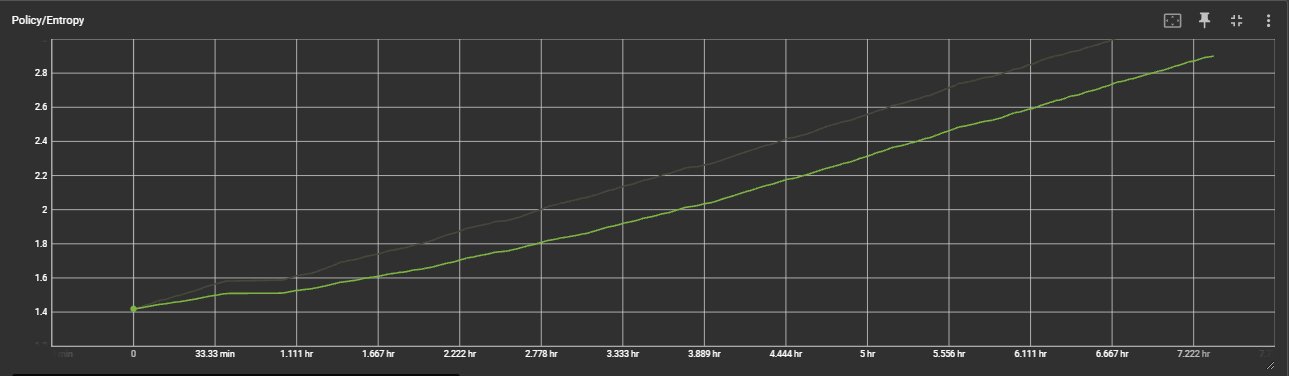
\includegraphics[width=0.8\textwidth]{Figures/App-YokosukaSearchEntropy.png}
  \caption{エントロピーの推移} 
  \label{fig:fig-01}
\end{figure}
\begin{figure}[H] 
  \centering 
  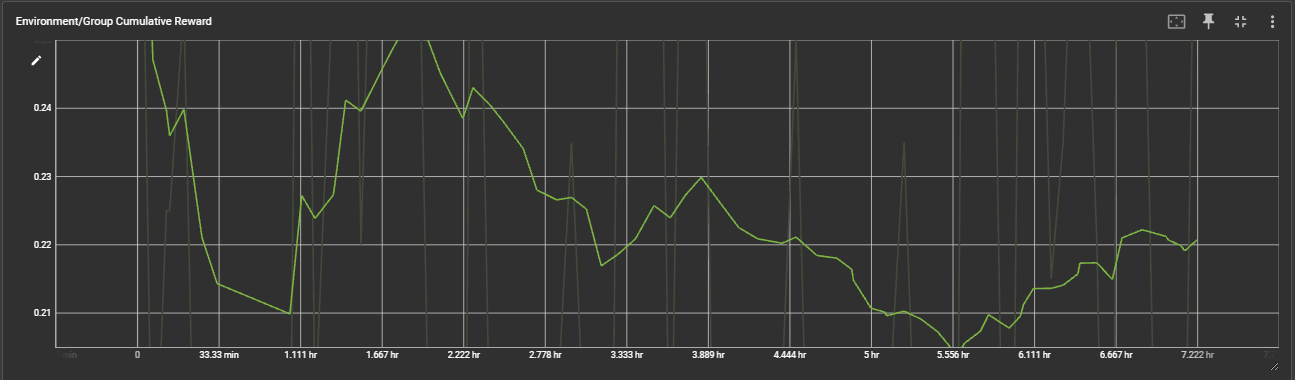
\includegraphics[width=0.8\textwidth]{Figures/App-YokosukaSearchGroupRward.png}
  \caption{グループ累積報酬の推移} 
  \label{fig:fig-01}
\end{figure}
\begin{figure}[H] 
  \centering 
  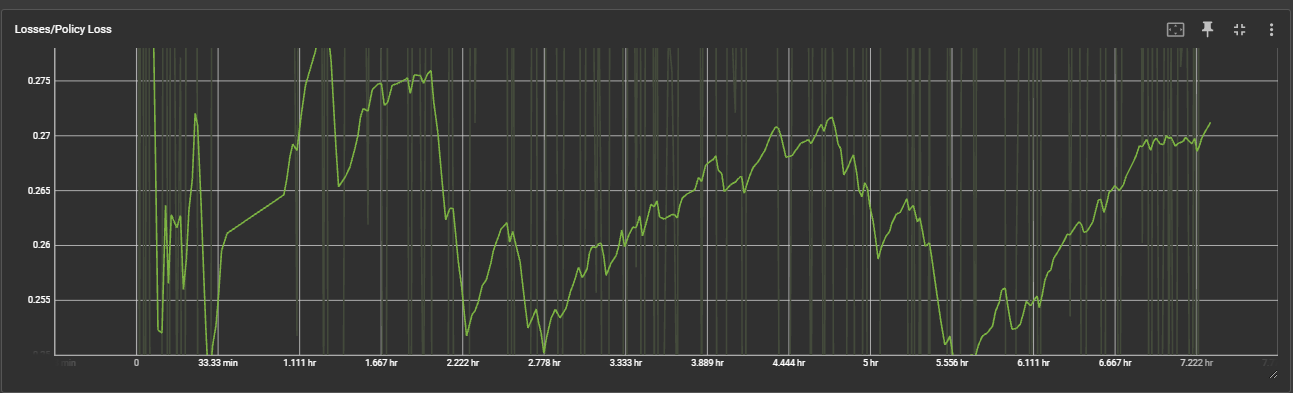
\includegraphics[width=0.8\textwidth]{Figures/YokosukaSearch-PolicyLoss.png}
  \caption{ポリシー関数の平均損失} 
  \label{fig:fig-01}
\end{figure}
\begin{figure}[H] 
  \centering 
  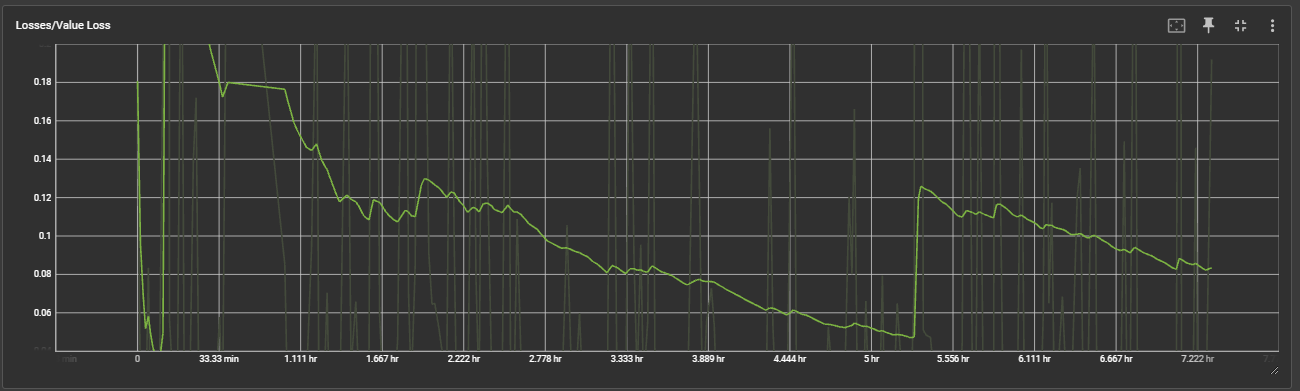
\includegraphics[width=0.8\textwidth]{Figures/App-YokosukaSearchVlueLoss.png}
  \caption{価値関数の平均損失} 
  \label{fig:fig-01}
\end{figure}


\subsection{沼津市の場合}
\begin{figure}[H] 
  \centering 
  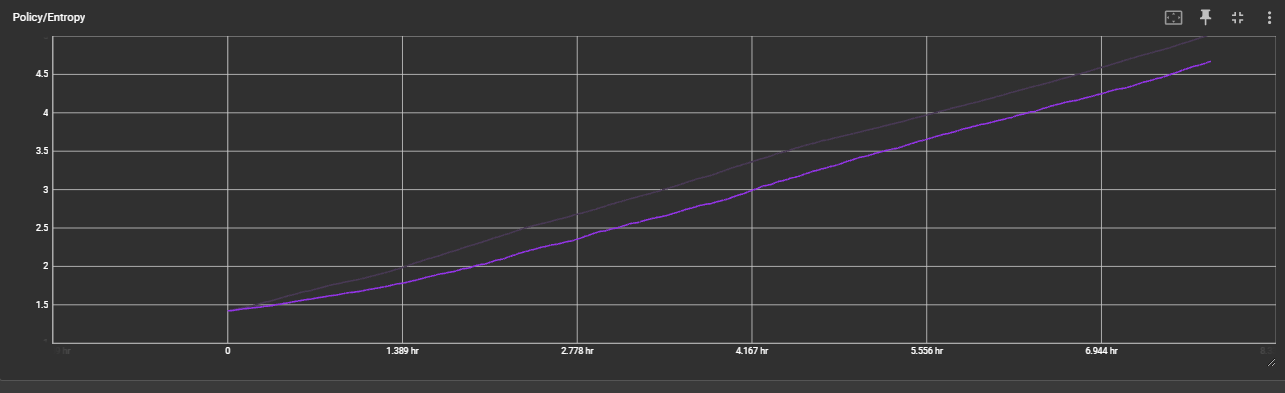
\includegraphics[width=0.8\textwidth]{Figures/NumazuSearch-Entropy.png}
  \caption{エントロピーの推移} 
  \label{fig:fig-01}
\end{figure}
\begin{figure}[H] 
  \centering 
  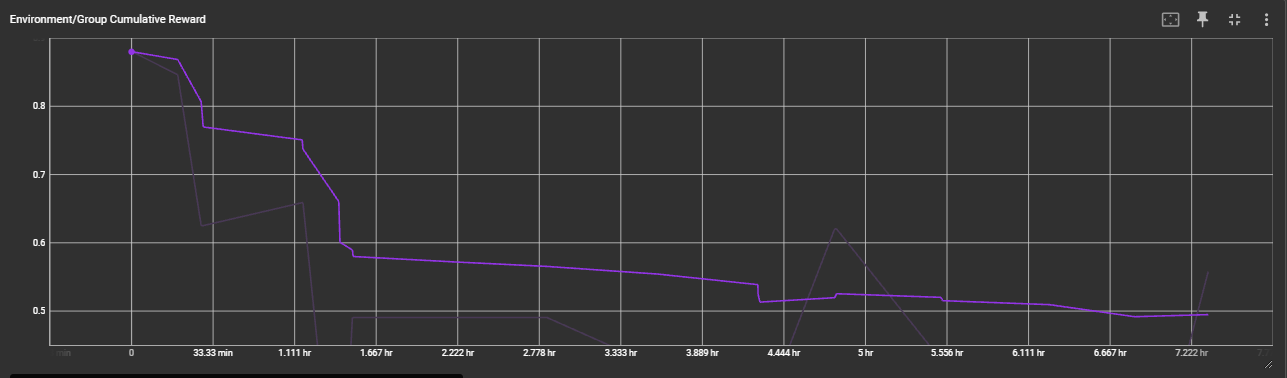
\includegraphics[width=0.8\textwidth]{Figures/NumazuSearch-GroupReward.png}
  \caption{グループ累積報酬の推移} 
  \label{fig:fig-01}
\end{figure}
\begin{figure}[H] 
  \centering 
  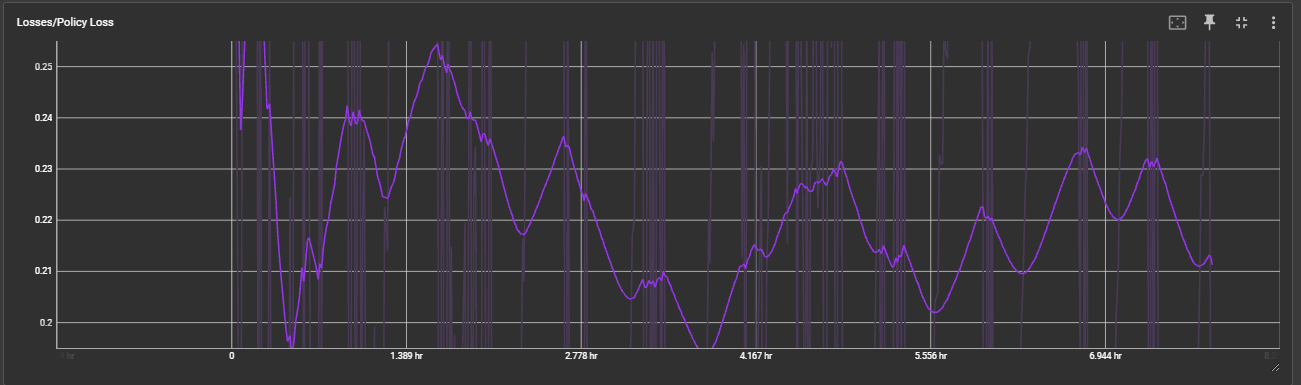
\includegraphics[width=0.8\textwidth]{Figures/NumazuSearch-PolicyLoss.png}
  \caption{ポリシー関数の平均損失} 
  \label{fig:fig-01}
\end{figure}
\begin{figure}[H] 
  \centering 
  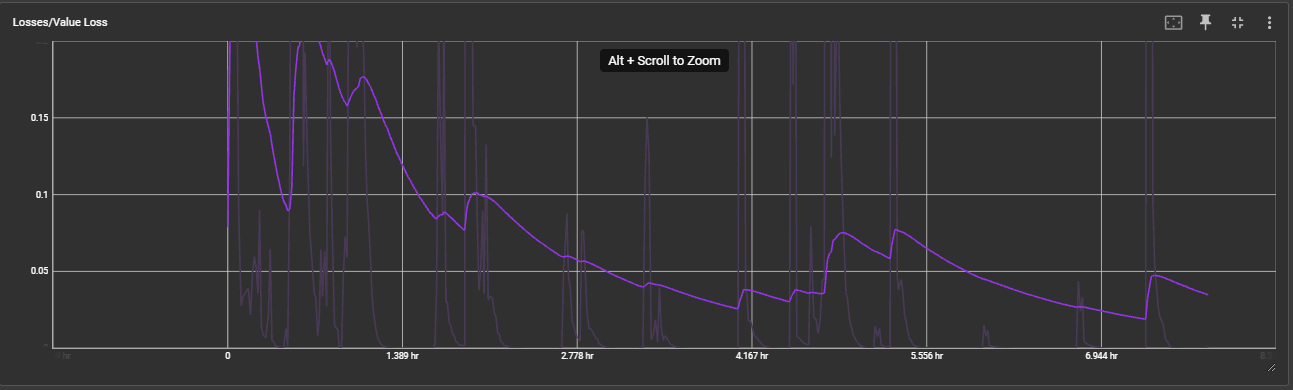
\includegraphics[width=0.8\textwidth]{Figures/NumazuSearch-ValueLoss.png}
  \caption{価値関数の平均損失} 
  \label{fig:fig-01}
\end{figure}

\section{誘導タスクマルチエージェントモデルの学習結果}

\subsection{横須賀市の場合}
\begin{figure}[H] 
  \centering 
  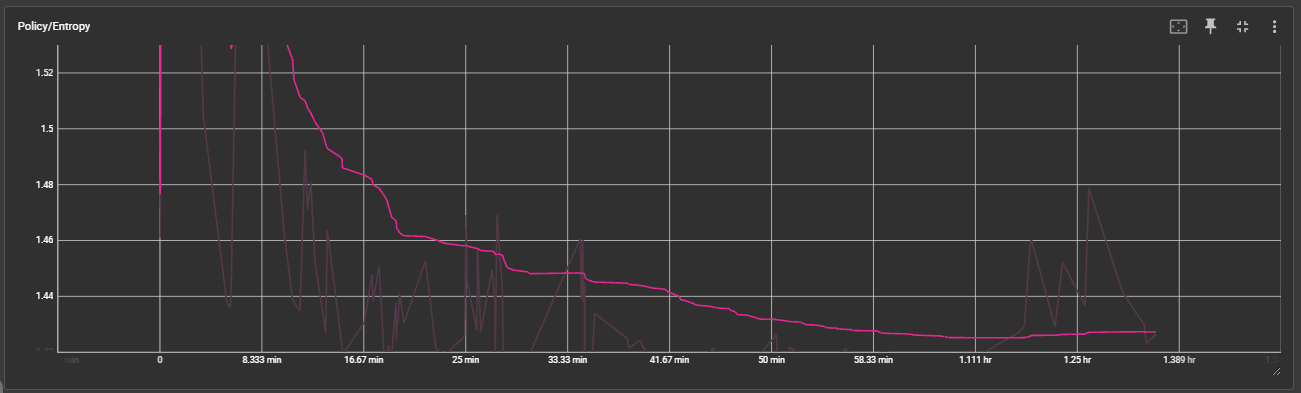
\includegraphics[width=0.8\textwidth]{Figures/Yokosuka-Entropy.png}
  \caption{エントロピーの推移} 
  \label{fig:fig-01}
\end{figure}
\begin{figure}[H] 
  \centering 
  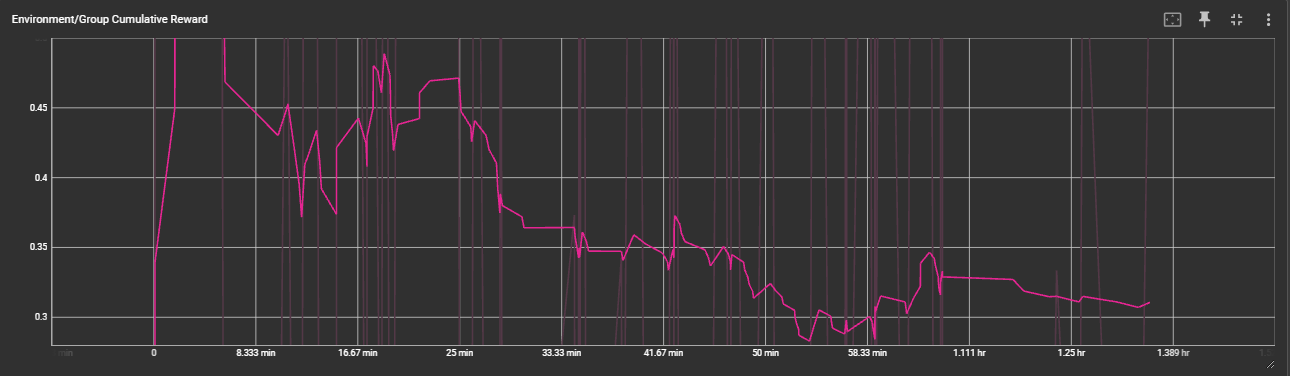
\includegraphics[width=0.8\textwidth]{Figures/Yokosuka-GroupReward.png}
  \caption{グループ累積報酬の推移} 
  \label{fig:fig-01}
\end{figure}
\begin{figure}[H] 
  \centering 
  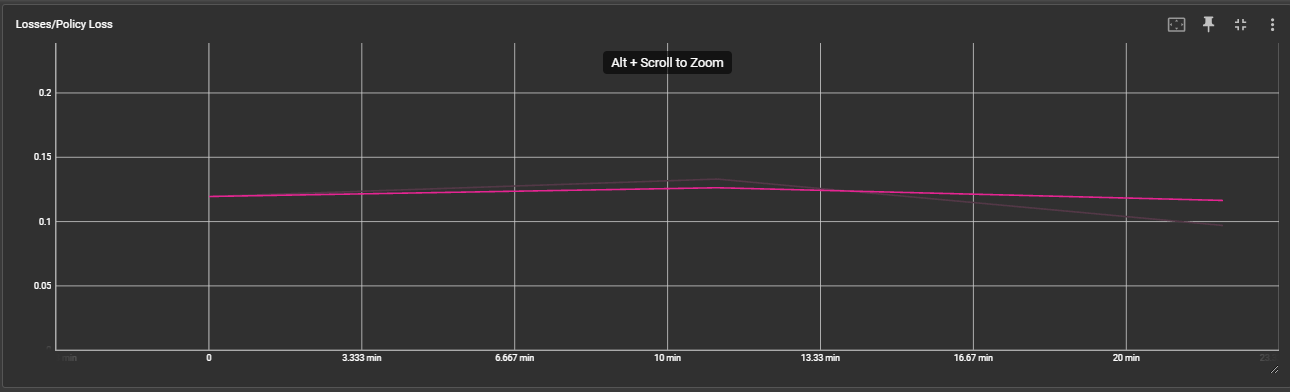
\includegraphics[width=0.8\textwidth]{Figures/Yokosuka-PolycyLoss.png}
  \caption{ポリシー関数の平均損失} 
  \label{fig:fig-01}
\end{figure}
\begin{figure}[H] 
  \centering 
  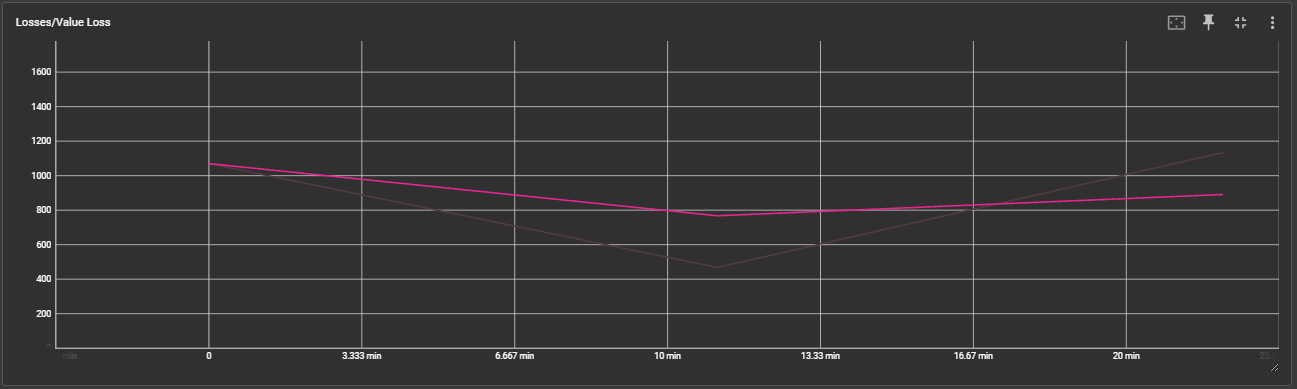
\includegraphics[width=0.8\textwidth]{Figures/YokosukaValueLoss.png}
  \caption{価値関数の平均損失} 
  \label{fig:fig-01}
\end{figure}


\subsection{沼津市の場合}
\begin{figure}[H] 
  \centering 
  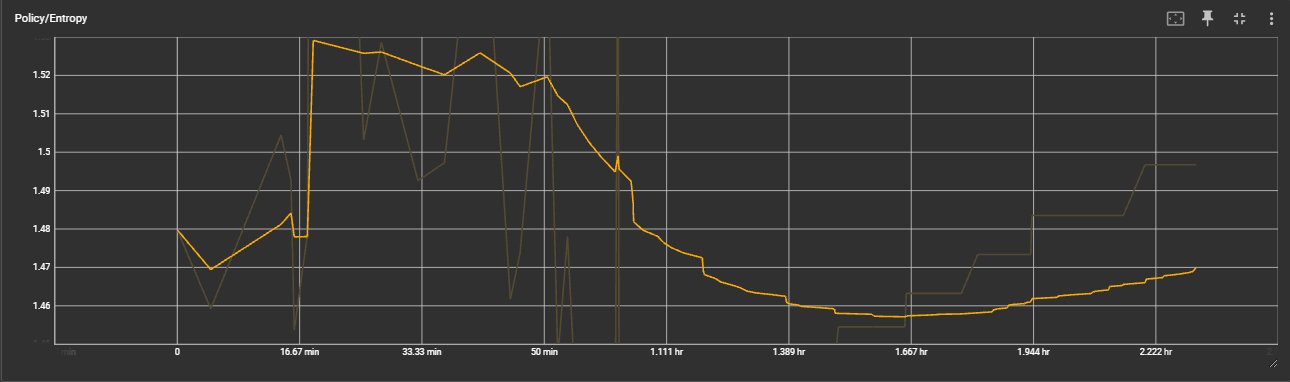
\includegraphics[width=0.8\textwidth]{Figures/NumazuEntropy.png}
  \caption{エントロピーの推移} 
  \label{fig:fig-01}
\end{figure}
\begin{figure}[H] 
  \centering 
  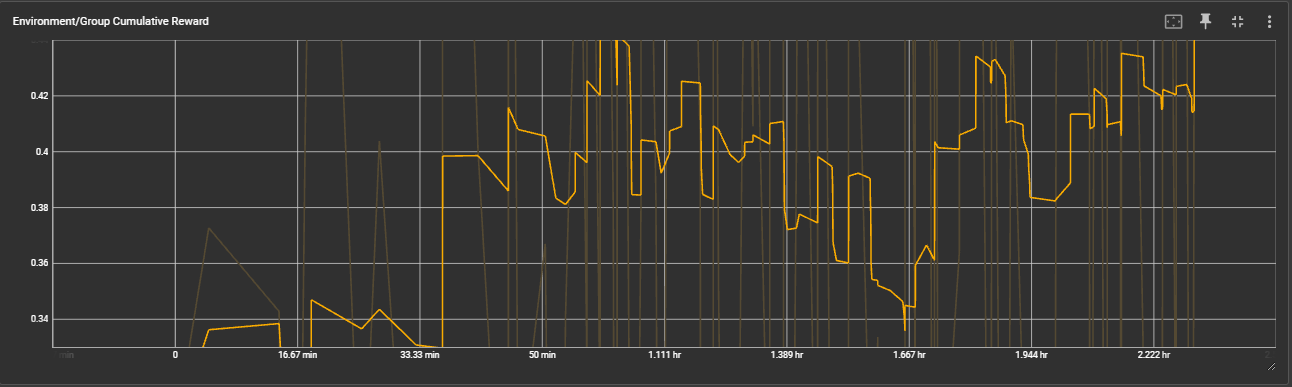
\includegraphics[width=0.8\textwidth]{Figures/NumazuGroupReward.png}
  \caption{グループ累積報酬の推移} 
  \label{fig:fig-01}
\end{figure}
\begin{figure}[H] 
  \centering 
  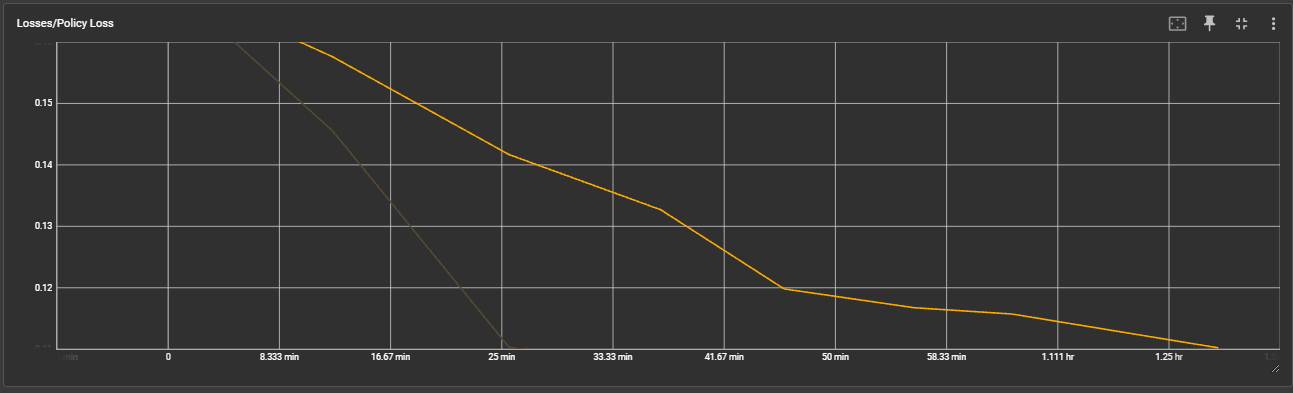
\includegraphics[width=0.8\textwidth]{Figures/NumazuPolicyLoss.png}
  \caption{ポリシー関数の平均損失} 
  \label{fig:fig-01}
\end{figure}
\begin{figure}[H] 
  \centering 
  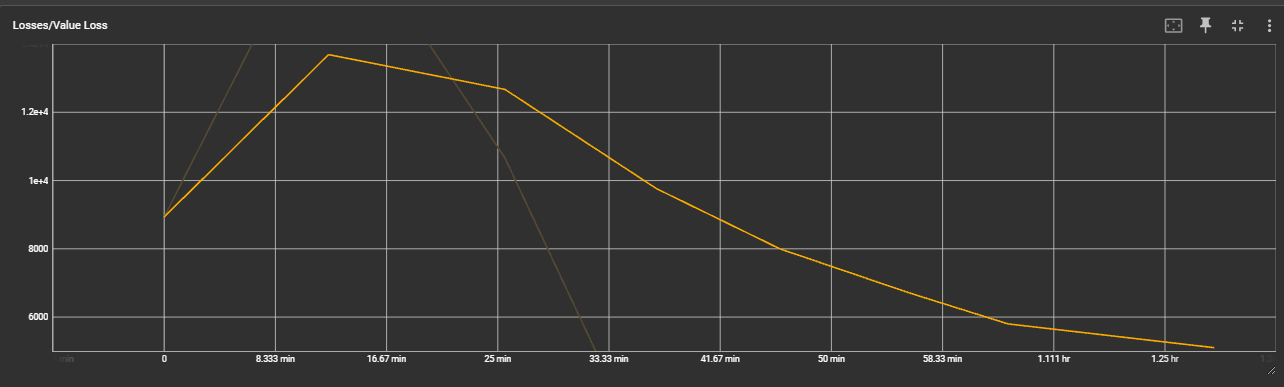
\includegraphics[width=0.8\textwidth]{Figures/NumazuValueLoss.png}
  \caption{価値関数の平均損失} 
  \label{fig:fig-01}
\end{figure}